\section{IoTDSL}
\label{sec:IoTDSL}

\begin{figure*}%
%\includegraphics[width=\columnwidth]{filename}%
\caption{Alice's Smart Home equipped with various devices.}%
\label{fig:RE}%
\end{figure*}

Building a well-calibrated \DSL is known to be difficult and error-prone. It usually requires a large expertise on a domain and its many variations before a consensus on which concepts are important and how to effectively represent them emerge. Fortunately, \MDE technologies operated substantial breakthrough over the past decade, allowing language designers to easily define their own \DSL structures and user interfaces. A \DSL is often required to exhibit a visual syntax, allegedly to simplify its understanding and manipulation by end-users. However, in order to obtain faster a functional prototype, we chose to start from a textual syntax, which is easier to manipulate and evolve for language designers. Ultimately, we plan to propose a visual syntax: the transition should be facilitated since our \DSL is developed from the start in GeMoC \cite{combemale-14}, an \textsc{Mde} framework that supports both visual and textual representations as concrete syntaxes and maintains a full synchronisation between both versions.



Based on the concerns and challenges identified in section~\ref{sec:Context-Challenges}, we now introduce \IOTDSL, our \DSL devoted to facilitate the high-level manipulation of \IOT systems. At the heart of \IOTDSL are two governing principles. First, we promote a clean separation of concerns for all aspects the \DSL has to handle. As a consequence, our \DSL's structure embeds several sublanguages that are composed together to form \IOTDSL. We believe this approach to be scalable, and to support a well-controlled independent evolution of each concern without impacting the other aspects, since those aspects are composed through well-defined interfaces. Second, our \DSL relies on events, a natural paradigm for specifying various models of interactions that is classically used in embedded and critical systems, and where a clear separation between the system and its environment is performed, helping us enforce separation of concerns.



Despite its early stages of development, \IOTDSL showed its ability to appropriately capture the definition of small-scale \IOT systems. We first extract a simple scenario from our project at the University of Namur to demonstrate typical usages of \IOT systems deployed inside a house. We then simultaneously explain each part of the definition of \IOTDSL, and illustrate it in dedicated examples.

\subsection{Running Example}
\label{sec:IoTDSL-Example}


<<<<<<< .mine
To illustrate our proposal, we consider a smart home equipped with several devices, just like Alice's situation in Section \ref{sec:Context-Challenges}, as illustrated in Figure \ref{fig:RE}. At the entrance, the door is equipped with a lock detector, allowing to know when the door is opened or closed. The hallway contains movement detectors, so that the lights in the hallway as well as in the living room automatically switch on when she enters her house. Furthermore, the living room also contains a presence detector because Alice wants the temperature to be automatically monitored when she's occupying the room, being maintained between 20°C and 22°C. Otherwise, when she is not home, the temperature may not go below 16°C. For security reasons, Alice's kitchen contains a smoke detector and a temperature monitor. When she cooks, it happens that she burns something; but she wants to make sure to detect any departing fire: she considers critical situations when the temperature remains above 45°C consistently during five minutes while there is also smoke in the kitchen. 
||||||| .r79
To illustrate our proposal, we consider a smart home equipped with several devices, just like Alice's situation in Section \ref{sec:Context-Challenges}, as illustrated in Figure \ref{fig:RE}. At the entrance, the door is equipped with a lock detector, allowing to know when the door is opened or closed. The hallway contains movement detectors, so that the lights in the hallway as well as in the living room automatically switch on when she enters her house. Furthermore, the living room also contains a presence detector because Alice wants the temperature to be automatically monitored when she's occupying the room, being maintained between 20°C and 22°C; otherwise, we she is not home, the temperature may not go below 16°C. For security reasons, Alice's kitchen contains a smoke detector and a temperature monitor. When she cooks, it happens that she burns something; but she wants to make sure to detect any departing fire: she considers it a critical situation when the temperature remains above 45°C consistently during five minutes while there is also smoke in the kitchen. 
=======
To illustrate our proposal, we consider a smart home equipped with several devices, just like Alice's situation in Section \ref{sec:Context-Challenges}, as illustrated in Figure~\ref{fig:RE}. At the entrance, the door is equipped with a lock detector, allowing to know when the door is opened or closed. The hallway contains movement detectors, so that the lights in the hallway as well as in the living room automatically switch on when she enters her house. Furthermore, the living room also contains a presence detector because Alice wants the temperature to be automatically monitored when she's occupying the room, being maintained between 20°C and 22°C; otherwise, when not at home, the temperature may not go below 16°C. For security reasons, Alice's kitchen contains a smoke detector and a temperature monitor. When she cooks, it happens that she burns something; but she wants to make sure to detect any departing fire: she considers it a critical situation when the temperature remains above 45°C consistently during five minutes while there is also smoke in the kitchen. 
>>>>>>> .r80

Figure \ref{fig:RE} shows how the various devices are physically distributed inside an archetypal representation of a smart home, and how each device communicates with a centralised gateway. In our \DSL, the gateway concentrates the data received from the devices deployed inside the home, and keeps the business logic running, \textit{i.e.} receiving data from and acting through the devices. 

\subsection{Type Definition}
\label{sec:IoTDSL-Type}

<<<<<<< .mine
In this section, we define \IOT devices' types, \textit{i.e.} which capabilities are available to the users in terms of environment sensing and actuating. In our scenario, type definitions either come from an advanced user who is able to properly reason about a particular device and extract the relevant information, or from a preexisting devices database, either being an actual database the system is connected to, or a library made available to users. From a metamodel point-of-view, this part is similar to the notion of \textsf{Classifier} in \textsc{Mof}-like languages: a \textsf{Type} is either a \textsf{PrimitiveType} (integer and real numbers, strings and booleans), or a user-defined \textsf{DeclaredType}. We distinguish between general \textsf{Gateway}s, which centralise information and processing, from \textsf{Node}s, which possess capabilities and are deployed in the environment. A \textsf{Capability} is basically a \textsc{Mof}-like operation with a signature, expressed through a list of (input/output typed) \textsf{Parameter}s that either captures data from the environment, or acts on it. A \textsf{Node} can mix both kinds of capabilities, allowing us to represent in a uniform fashion composite devices that expose complex behaviours.
||||||| .r79
In this section, we define \IOT devices' types, \textit{i.e.} which capabilities are available to the user in terms of environment sensing and actuating. In our scenario, type definitions either come from an advanced user who is able to properly reason about a particular device and extract the relevant information, or from a preexisting devices database, either being an actual database the system is connected to, or a library made available to users. From a metamodel point-of-view, this part is similar to the notion of \textsf{Classifier} in \textsc{Mof}-like languages: a \textsf{Type} is either a \textsf{PrimitiveType} (integer and real numbers, strings and booleans), or a user-defined \textsf{DeclaredType}. We distinguish between general \textsf{Gateway}s, which centralise information and processing, from \textsf{Node}s, which possess capabilities and are deployed in the environment. A \textsf{Capability} is basically a \textsc{Mof}-like operation with a signature, expressed through a list of (input/output typed) \textsf{Parameter}s that either captures data from the environment, or acts on it. A \textsf{Node} can mix both kinds of capabilities, allowing us to represent in a uniform fashion composite devices that expose complex behaviours.
=======
\begin{figure*}%
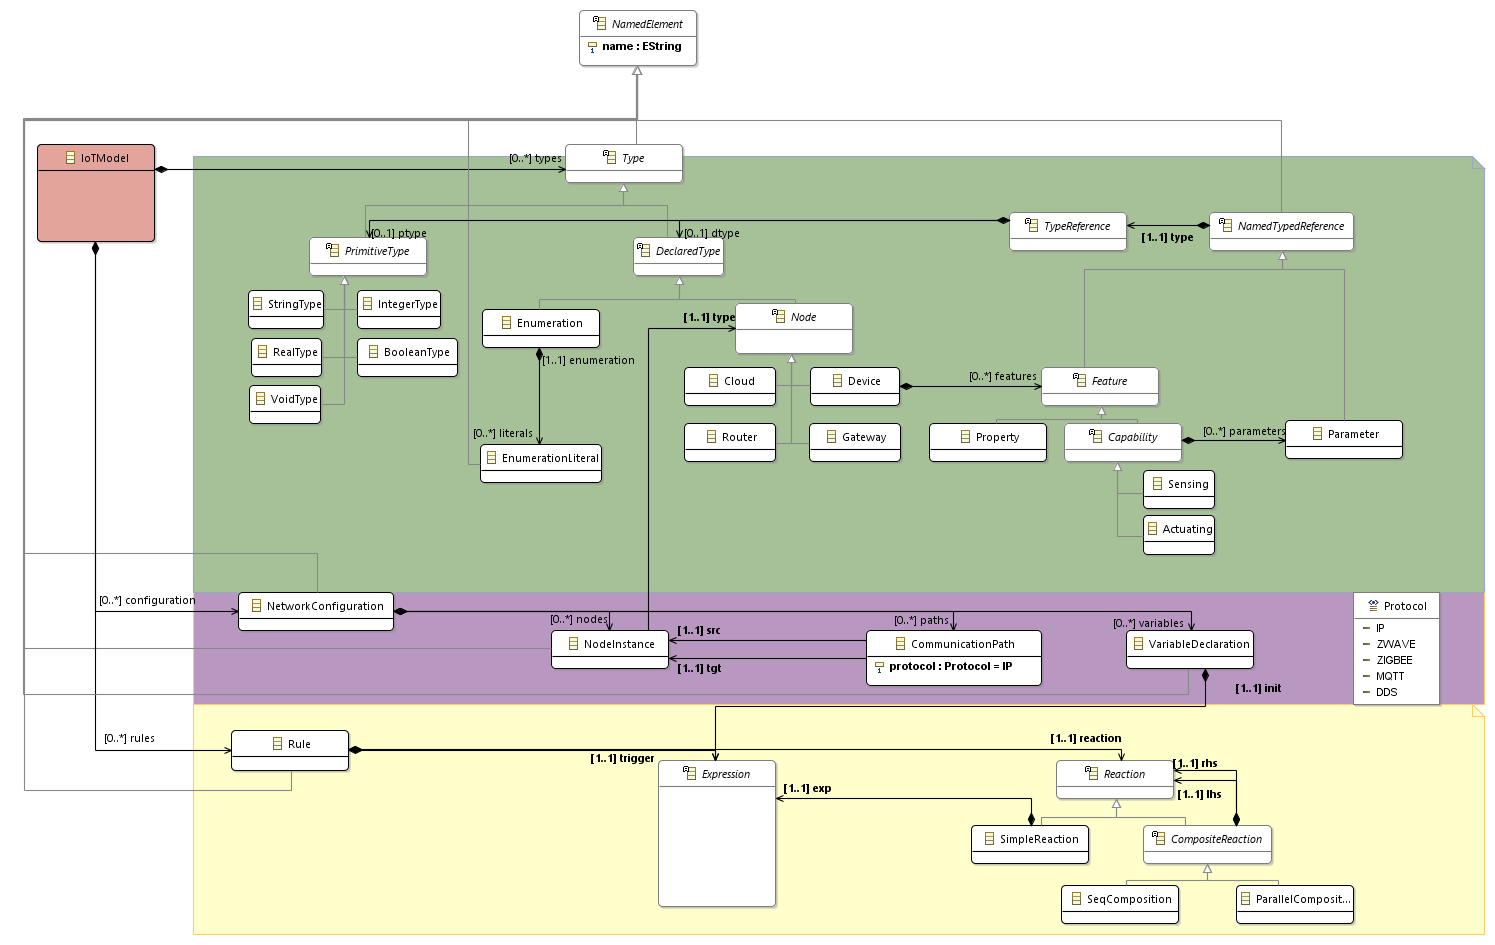
\includegraphics[width=\textwidth]{IoTDevice}%
\caption{Metamodel of \IOTDSL, separated in three concerns: in green, \emph{Type Definition} captures devices' capabilities; in purple, \emph{Network Configuration} details how device instances are connected to each others; and in yellow, \emph{Business Rules} defines the functionalities expected from the IoT installation.}%
\label{fig:IoTDevice-MM}%
\end{figure*}

In this section, we define \IOT devices' types, \textit{i.e.} which capabilities are available to the user in terms of environment sensing and actuating. In our scenario, type definitions either come from an advanced user who is able to properly reason about a particular device and extract the relevant information, or from a preexisting devices database, either being an actual database the system is connected to, or a library made available to users. Figure \ref{fig:IoTDevice-MM} (green) shows the metamodel part dedicated to type definitions. From a language point-of-view, this part is similar to the notion of \textsf{Classifier} in \textsc{Mof}-like languages: a \textsf{Type} is either a \textsf{PrimitiveType} (integer and real numbers, strings and booleans), or a user-defined \textsf{DeclaredType}. We distinguish between general \textsf{Gateway}s, which centralise information and processing, from \textsf{Node}s, which possess capabilities and are deployed in the environment. A \textsf{Capability} is basically a \textsc{Mof}-like operation with a signature, expressed through a list of (input/output typed) \textsf{Parameter}s that either captures data from the environment, or acts on it. A \textsf{Node} can mix both kinds of capabilities, allowing us to represent in a uniform fashion composite devices that expose complex behaviours.
>>>>>>> .r80
	
For now, type definitions are defined as specific files that can be imported and combined easily within an \IOT specification. Ultimately, we will propose a graphical interface that would facilitate the browsing of library components and their seamless integration into \IOT systems.

Figure \ref{fig:RE-TypeDeclarations} shows how the devices used in the Running Example are declared in \IOTDSL: each device is introduced by the keyword \textsf{device}, has a name and capabilities that correspond to reporting events (\textsf{sensing}) or operating over the environment (\textsf{actuating}). A special device, introduced by the keyword \textsf{gateway}, centralises data from all devices connected to it (cf. Section \ref{sec:IoTDSL-NetworkConfiguration}). Note that this is the visible part of \IOTDSL: in the background, the events declared for all devices need to be mapped to concrete low-level events that the devices actually use. For that purpose, \IOTDSL contains a mapping language aimed at reconciling high- and low-level events that is not detailed here for space reasons.

\begin{figure}[t]%
	\begin{boxedminipage}[t]{\columnwidth}
	\begin{sffamily}
		\begin{tiny}
		\begin{minipage}[t]{0.5\columnwidth}
\textbf{device} DoorLock\{\\
   \phantom{M}\textbf{sensing} opened()\\
   \phantom{M}\textbf{sensing} closed()\\
\}\\
\textbf{device} PresenceDetector\{\\
   \phantom{M}\textbf{sensing} detected()\\
   \phantom{M}\textbf{actuating} isPresent()\\
\}\\
\textbf{device} LightBulb\{\\
   \phantom{M}\textbf{actuating} on()\\
   \phantom{M}\textbf{actuating} off()\\
   \phantom{M}\textbf{actuating} blink()\\
\}\\	
\textbf{device} TempSensor \{\\
   \phantom{M}\textbf{sensing} getTemp( )\\
\}
		\end{minipage}
		\hfill
		\begin{minipage}[t]{0.45\columnwidth}
\textbf{device} Heater\{\\
\phantom{M}\textbf{actuating} warm(delay:Integer)\\
\phantom{M}\textbf{actuating} stop()\\
\}\\
\textbf{device} Alarme\{\\
   \phantom{M}\textbf{actuating} sound()\\
   \phantom{M}\textbf{actuating} call(msg:String)\\
\}\\
\textbf{device} Timer\{\\
   \phantom{M}\textbf{actuating} reset()\\
   \phantom{M}\textbf{actuating} set(delay:Integer)\\
   \phantom{M}\textbf{sensing}   timeout()\\
\}\\\\
\textbf{gateway} Central\\		
		\end{minipage}
		\end{tiny}
	\end{sffamily}
	\end{boxedminipage}

	\caption{Type Declarations in \IOTDSL: Devices declare capabilities (i.e. sensing or actuating) as high-level events to be manipulated by end-users.}%
	\label{fig:RE-TypeDeclarations}%
\end{figure}



	
\subsection{Network Configuration}
\label{sec:IoTDSL-NetworkConfiguration}

This part defines how devices are connected (cf. Figure \ref{fig:IoTDevice-MM}, purple): an actual device within a system is represented by a \textsf{NodeInstance} and is typed by a \textsf{Node} or a \textsf{Gateway}; instances communicate with other \IOT devices or gateways through predefined \textsf{CommunicationPath}s: such a path defines, among other information, the protocol(s) used for communication. We rely on existing platforms such as OpenRemote or SmartThings to handle the communication protocols intricate details, since those details are, from an end-user viewpoint, technical aspects rather than essential matters. By knowing which protocols are used between each pair of devices, we can perform data conversion in the proper format required by the protocols automatically: most of those protocols are already implemented in General-Purpose Programming Languages (\textsc{Gpl}s), like Java or C, to name a few of them.
	
\begin{figure}[t]%
	\begin{boxedminipage}[t]{\columnwidth}
	\begin{sffamily}
		\begin{tiny}
		{\setlength{\baselineskip}{1.2\baselineskip}
\textbf{configuration} MyHome\{\\
   \phantom{M}\textbf{node} gw \textbf{:} Central\\
   \phantom{M}\textbf{node} livingTemp  \textbf{:} TemperaturSensor\\
   \phantom{M}\textbf{node} kitchenTemp \textbf{:} TemperaturSensor\\
   \phantom{M}\textbf{node} livingHeater  \textbf{:} Heater\\
   \phantom{M}\textbf{node} frontdoor     \textbf{:} DoorLock\\
   \phantom{M}\textbf{node} corridorLight \textbf{:} LightBulb\\
	\phantom{M}\textbf{node} livingLight   \textbf{:} LightBulb\\
   \phantom{M}\textbf{node} timer  \textbf{:} Timer\\
   \phantom{M}\textbf{node} alarme \textbf{:} Alarme\\
   \phantom{M}\textbf{node} corridorDetector\textbf{:} PresenceDetector\\
	\phantom{M}\textbf{node} livingDetector  \textbf{:} PresenceDetector
	\\\\
   \phantom{M}\textbf{from} livingTemperature  \textbf{to} gw \textbf{via} MQTT\\
   \phantom{M}\textbf{from} HomeTemperature \textbf{to} gw \textbf{via} DDS\\
   \phantom{M}\textbf{from} livingHeater   \textbf{to} gw \textbf{via} DDS\\
   \phantom{M}\textbf{from} frontdoor  \textbf{to} gw \textbf{via} MQTT\\
   \phantom{M}\textbf{from} light \textbf{to} gw \textbf{via} MQTT\\
   \phantom{M}\textbf{from} timer \textbf{to} gw \textbf{via} DDS\\
   \phantom{M}\textbf{from} alarme \textbf{to} gw \textbf{via} DDS\\
   \phantom{M}\textbf{from} bodydetector  \textbf{to} gw \textbf{via} MQTT\\
\}
	\par}
		\end{tiny}
	\end{sffamily}
	\end{boxedminipage}
	\caption{Network Configuration for the devices present in Alice's House}%
	\label{fig:RE-Network}%
\end{figure}	

From a practical viewpoint, we can easily imagine that network configurations are automatically established if devices follow the recommendation of discovery protocols (cf. \cite{} for an overview). By concentrating the connections on a gateway in charge of centralising the upcoming or leaving devices, e.g., phones that enter or leave a house, or devices that (dis)connect, it becomes possible to gather information on new devices and connect them appropriately to other devices in the network according to their capabilities, communication protocols, and so on.

Figure \ref{fig:RE-Network} shows the connection between devices, as illustrated in Figure \ref{fig:RE}: a specific device is considered as an instance of a type, as declared in Section \ref{sec:IoTDSL-Type}, which allows to distinguish various devices with the same set of capabilities through identifiable references (reference names are just here for illustration purposes); the communication is purely declarative and only mentions the protocol type (after the \textsf{via} keyword). Note that this configuration introduces an extra instance \textsf{timer:Timer} used to simulate time elapse: this allows us to artificially introduce time through a specific ``fake'' device, whose behaviour is linked directly to the gateway's supporting platform for time management.


	
\subsection{Business Rules}
\label{sec:IoTDSL-BusinessRules}

This last part of our \DSL is the heart of \IOT systems manipulation (cf. Figure \ref{fig:IoTDevice-MM}, yellow). It relies on an event-based framework consisting of a set of \textsf{Rule}s that implements various functionalities the end-user wants to achieve: rules' \textsf{trigger}s are cyclically evaluated against the surrounding environment, whenever a \textsf{trigger} \textsf{Expression} becomes true, it executes the appropriate \textsf{reaction} associated to the rule. A \textsf{trigger} is defined by an expression, whose precise definition is omitted here, since it simply follows classical expression languages from any \textsc{Gpl} for navigating nodes, and evaluating boolean and arithmetic expressions\footnote{Note that detecting the \emph{absence} of events is left for future work, since this is a rather tricky problem, as a consequence, the current expression language does not integrate boolean negation yet.}.A \textsf{reaction} defines a sequential or parallel combination of capabilities, allowing to order an action by, or to require a data from some identifiable devices. For example, a \textsf{reaction} may be to make blinking all lights in a house, or only the ones a certain type.
	
For now, our approach is purely centric: rules are gathered into a gateway. For efficiency and resource consumption reasons, we are also exploring how to automatically identify parts of the business logics that can be deported into specific nodes with sufficient processing and power resources, in order to communicate through the network the information that is truly relevant for other devices.

We now explain how the scenario of the running example are translated in business rules in \IOTDSL. We identified three different situations where Alice needs to specify what she expects from the devices of her house:
\begin{enumerate}
	\item When Alice enters home (and thus opens the front door), she wants the lights in the hallway and the living room to automatically switch on. 

	\noindent
	
	\begin{small}	
		\begin{sffamily}
	\textbf{rule} SwitchLightsWhenEnter:\\
	\phantom{M}\textbf{when} (frontdoor.opened() \textbf{and after}\\
	\phantom{MMMM} corridorDetector.detected()) \textbf{do} \{\\
	\phantom{MM} corridorLight.on() \textbf{||} livingLight.on()\\ 			
	\phantom{M} \}
		\end{sffamily}
	\end{small}
	
	\item When Alice is in the living room, the temperature inside the room should be maintained between comfortable temperatures; whereas when she is not, the temperature should not drop below 16°C.
	
		\noindent
	
	\begin{small}	
		\begin{sffamily}
	\textbf{rule} PresentInLiving:\\	
	\phantom{M}\textbf{when} (presenceTimer.timeout()) \textbf{do}\{\\
	\phantom{MM} livingDetector.isPresent() \textbf{||}\\
	\phantom{MM} (presenceTimer.reset \textbf{;}\\ 
	\phantom{MML} presenceTimer.set(TIMEDETECT))\\
	\phantom{M}\}\\
	\textbf{rule} MonitorLivingTempInStop:\\
	\phantom{M}\textbf{when} (livingDetector.detected() \textbf{and}\\
	\phantom{MMMM} livingTemp.getTemp > IN\_MAX) do \{\\
	\phantom{MM} livingHeater.stop()\\ 			
	\phantom{M}\}\\
	\textbf{rule} MonitorLivingTempInStart:\\
	\phantom{M}\textbf{when} (livingDetector.detected() \textbf{and}\\
	\phantom{MMMM} livingTemp.getTemp < IN\_MIN) do \{\\
	\phantom{MM} livingHeater.warm(TIMEHEAT)\\ 			
	\phantom{M}\}\\
	\textbf{rule} MonitorLivingTempOutStart:\\
	\phantom{M}\textbf{when} (presenceTimer.timeout() \textbf{before} \textbf{and}\\
	\phantom{MMMM} livingTemp.getTemp < OUT\_MIN) do \{\\
	\phantom{MM} livingHeater.warm(TIMEHEAT)\\ 			
	\phantom{M}\}\\
		\end{sffamily}
	\end{small}
	
	\item There is a critical fire situation when smoke is detected in the kitchen while temperature is maintained beyong 45°C for at least five minutes.
\end{enumerate}

These rules show some specificities of \IOTDSL's Rule language. First, it is possible to define local or global variables and reuse them as part of parameters or expressions (cf. Rules \textsf{PresentInLiving} or \textsf{MonitorLivingInStop}, among others). Second, it is possible to compose reactions either in sequence (Class \textsf{SeqComposition} in the metamodel of Figure \ref{fig:IoTDevice-MM}, textually represented as \textsf{\textbf{;}}) or in parallel (Class \textsf{ParallelComposition}, represented as \textsf{\textbf{||}}), like Rule \textsf{PresentInLiving} demonstrates. Third, \IOTDSL's expression language integrates a simple mechanism for events time management: the \textsf{before} and \textsf{after} event modifiers check that an event happens in a reasonable time windows before/after the one it is combined to (in Rules \textsf{SwitchLightWhenEnter} and \textsf{MonitorLivingTempOutStart}, events are combined with \textsf{and} for checking quasi-simultaneity). Fourth, because \IOTDSL cannot check the non-occurence of events, time management is crucial for ensuring a sound detection of interesting non-events: for example here, Rule \textsf{PresentInLiving} is used to periodically check for presence in the living room (with the actuation \textsf{isPresent()}); but when nobody is detected, we still have to maintain the temperature above \textsf{OUT\_MIN} = 16°C. By detecting that \textsf{timeout()} occured previously, we still are capable of adjusting the living room temperature adequately.
